\chapter{Konfigurieren des TransistorTesters}
\label{sec:config}
Die ganze Software des TransistorTesters ist im Quellcode verfügbar.
Die Übersetzung der Module wird mit einer Makefile gesteuert. Die Entwicklung wurde
auf einen Ubuntu Linux Betriebssystem mit den GNU-Werkzeugen (GNU toolchain, gcc version 4.5.3) durchgeführt.
Es sollte möglich sein, ohne Schwierigkeiten andere Linux-Betriebssysteme zu benutzen.
Um die übersetzen Daten in den Flash-Speicher oder den EEprom-Speicher zu laden, wird das
Programm avrdude \cite{avrdude} (Version 5.11svn) von der Makefile benutzt, wenn man ,,make upload'' aufruft.
Das Programm avrdude ist für Linux und Windows verfügbar.
Der GNU C-Kompiler wird auch von der AVR-studio-Software unter Windows oder von
der WinAVR \cite{winavr1},\cite{winavr2} Software benutzt.
Sie können die Programmdaten (.hex und .eep) auch mit anderen Programmen in den ATmega laden,
aber nur meine Makefile Version stellt sicher, dass die richtigen Daten in den gewählten Prozessor gelangen.
Avrdude lädt Daten nur in den ATmega, wenn die Signaturbytes des angeschlossenen ATmega gleich mit dem ausgewählten sind.
Wenn Sie die Makefile ändern, wird die Software komplett neu übersetzt, wenn man ,,make'' oder
,,make upload'' aufruft.
Die Software, die für einen ATmega8 übersetzt wurde, läuft nicht auf einem ATmega168.
Die Software, die für einen ATmega328 übersetzt wurde, läuft nicht auf einem ATmega168.
Eine Ausnahme bildet Software, die für einen ATmega168 übersetzt wurde. Diese Programmdateien
sind auch für einen ATmega328 brauchbar.
Sind Sie vorsichtig, wenn Sie nicht das mitgelieferte Makefile benutzen.

Mit den entsprechenden Optionen ist die Software auch auf dem unveränderten Hardware-Entwurf von
Markus F. lauffähig (PARTNO=m8 , {\bf keine} NO\_AREF\_CAP und {\bf keine} PULLUP\_DISABLE Option).
Die Taktrate kann mit den fuses auch auf 8MHz gestellt werden, dazu ist kein Quarz erforderlich!


Die folgenden Optionen der Makefile sind verfügbar, um die Software für den Tester zu konfigurieren:

\begin{description}
  \item[PARTNO] beschreibt den Ziel-Prozessor:\\
         m8 = ATmega8\\
         m168 or m168p = ATmega168\\
         m328 or m328p = ATmega328\\
    Beispiel: PARTNO = m168
  \item[UI\_LANGUAGE] gibt die Sprache für den Tester an:\\
    LANG\_ENGLISH, LANG\_GERMAN, LANG\_POLISH, LANG\_CZECH, LANG\_SLOVAK, LANG\_SLOVENE und LANG\_DUTCH sind derzeit verfügbar.\\
    Beispiel: UI\_LANGUAGE = LANG\_ENGLISH
  \item[LCD\_CYRILLIC] wird nur gebraucht, wenn man ein LCD-Display mit kyrillischem Zeichensatz benutzt.
Die Zeichen \(\mu\) und \(\Omega\) sind im kyrillischen Zeichensatz nicht enthalten.
Wenn Sie diese Option angeben, werden beide Zeichen von der Software in das LCD geladen.\\
Beispiel: CFLAGS += -DLCD\_CYRILLIC
  \item[STRIP\_GRID\_BOARD] Diese Option passt die Software an eine andere Pinbelegung von Port~D für Streifenleiterplatinen an.
Die Einzelheiten findet man im Hardwarekapitel \ref{sec:hardware}.
  \item[WITH\_SELFTEST] Wenn Sie diese Option angeben, baut die Software eine Selbsttest-Funktion ein, die gestartet wird
wenn Sie alle drei Prüfspitzen verbinden und eine Messung starten.\\
Beispiel: CFLAGS += -DWITH\_SELFTEST
  \item[AUTO\_CAL] Der Nullabgleich für die Kondensatormessung und der Innenwiderstand der Port-Ausgänge wird beim
Selbsttest zusätzlich ins EEprom geschrieben und ist damit für die weiteren Messungen abgeglichen.
Wenn nach dem Nullabgleich der Kondensatormessung ein Kondensator mit einer Kapazität zwischen \(100 nF\) und \(20 \mu F\) an Pin~1 und Pin~3 
angeschlossen wird, wird auch der Offset des analogen Komparators und die Skalierung für die AUTOSCALE\_ADC
Umschaltung auf die interne Spannungsreferenz ermittelt und ins EEprom geschrieben.\\
Beispiel: CFLAGS += -DAUTO\_CAL
  \item[FREQUENCY\_50HZ] Zum Ende des Selbsttests wird bis zu einer Minute lang ein 50 Hz Signal auf Port 2 und Port 3 erzeugt.\\
Beispiel: CFLAGS += -DFREQUENCY\_50HZ
  \item[CAP\_EMPTY\_LEVEL] Diese Option legt die Spannung (mV) für einen entladenen Kondensator fest.
Der Wert kann höher als 3mV gesetzt werden, wenn die Entladung nicht zum Ende kommt. In diesen Fall meldet der Tester nach längerer Zeit ,,Cell!''.\\
Beispiel: CFLAGS += -DCAP\_EMPTY\_LEVEL=3
  \item[WITH\_AUTO\_REF] Mit dieser Option wird die Referenzspannung gemessen, um den aktuellen Faktor für die Kapazitätsmessung 
von kleineren Kapazitäten (unter \(40\mu F\)) zu ermitteln.\\
Beispiel: CFLAGS += -DWITH\_AUTO\_REF
  \item[REF\_C\_KORR] gibt einen Offset für die gelesene Referenz-Spannung in mV-Einheiten an.
Das kann benutzt werden, um die Kapazitätsmessung kleiner Kondensatoren abzugleichen.
Wenn zusätzlich die AUTO\_CAL Option gewählt wurde, ist diese Angabe nur ein zusätzlicher Offset für
den gefundenen Komparator-Offset.
Ein Wert von 10 ergibt etwa 1~Prozent kleinere Messergebnisse.\\
Beispiel: CFLAGS += -DREF\_C\_KORR=14
  \item[C\_H\_KORR] gibt eine Korrektur der Messergebnisse für grosse Kondensatoren an.
Eine Eingabe von 10 führt zu 1~Prozent kleineren Messergebnissen.\\
Beispiel: CFLAGS += -DC\_H\_KORR=10
  \item[AUTOSCALE\_ADC] schaltet die automatische Bereichswahl des ADC (entweder VCC oder interne Referenz) ein.
Die interne Referenz hat 2,56V für den ATmega8 und 1,1V für die anderen Prozessoren.\\
Beispiel: CFLAGS += -DAUTOSCALE\_ADC
  \item[ESR\_ZERO] gibt einen Nullwert für die ESR-Messung von Kondensatoren vor. Dieser Nullwert wird von den
ermittelten Messwerten abgezogen. Bei negativen ESR-Werten wird die Ausgabe ,,ESR=0?'' angezeigt und der Nullwert
im EEprom korrigiert. Dieser korrigierte Wert wird bei den folgenden Messungen wirksam, bis er wieder beim nächsten
Selbsttest zurückgesetzt wird.
Falls Sie immer zu hohe ESR-Werte messen, sollten Sie diesen Vorgabewert erhöhen.\\
Beispiel: CFLAGS += -DESR\_ZERO=29
  \item[NO\_AREF\_CAP] teilt der Software mit, dass Sie keinen Kondensator am AREF Pin (Pin 21) angeschlossen haben.
Dies ermöglicht kürzere Wartezeiten für die AUTOSCALE\_ADC Umschaltung des ADC.
Ein 1nF Kondensator wurde in diesem Modus ohne Fehler getestet.
Die Abbildungen~\ref{pic:aref1} und \ref{pic:aref5} zeigen die Schaltzeiten mit einem 1nF Kondensator.
Wie Sie sehen können ist das Schalten von 5V auf 1,1V viel langsamer als das Zurückschalten auf 5V.
Wenn Sie noch einen \(100 nF\) installiert haben, ist die Schaltzeit etwa Faktor 100 länger!\\
Beispiel: CFLAGS += -DNO\_AREF\_CAP

\end{description}

\begin{figure}[H]
  \begin{subfigure}[b]{9cm}
    \centering
    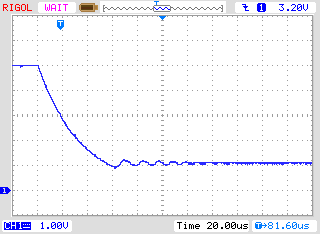
\includegraphics[width=9cm]{../PNG/AREF2_1V.png}
    \caption{from 5V to 1.1V }
    \label{pic:aref1}
  \end{subfigure}
  ~
  \begin{subfigure}[b]{9cm}
    \centering
    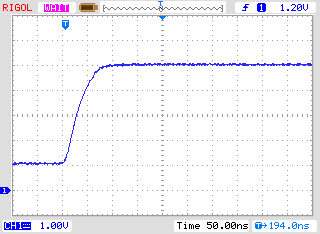
\includegraphics[width=9cm]{../PNG/AREF2VCC.png}
    \caption{from 1.1V to 5V}
    \label{pic:aref5}
  \end{subfigure}
  \caption{Umschalten von AREF mit einem \(1nF\) Kondensator}
\end{figure}

\begin{description}
  \item[REF\_R\_KORR] gibt einen Offset für die interne Referenz-Spannung in mV-Einheiten an.
Mit diesem Offset kann eine Differenz bei der Umschaltung der Referenzspannung für die Widerstandsmessung abgeglichen werden.
Wenn die AUTO\_CAL Option gewählt wurde, ist dieser Wert nur ein Offset zu der gefundenen Spannungs-Differenz in der
AUTO\_CAL Funktion.\\
Beispiel: CFLAGS += -DREF\_R\_KORR=10
  \item[OP\_MHZ] gibt der Software an, mit welcher Taktfrequenz in MHz der Tester arbeiten wird.
Die Software ist nur mit 1MHz, 8MHz und zusätzlich auch 16MHz getestet. Der Betrieb mit 8MHz wird wegen der besseren Auflösung der
Kondensator- und Spulen-Messung empfohlen.\\
Beispiel: OP\_MHZ = 8
  \item[RESTART\_DELAY\_TICS] muß auf 6 gesetzt werden, wenn der ATmega168 oder ATmega328 ohne Quarz mit dem
RC-Generator betrieben wird. Wenn dieser Wert nicht vorbesetzt wird, wählt die Software die 16384 Takte Startverzögerung für
den Quarzbetrieb.\\
Beispiel: CFLAGS += -DRESTART\_DELAY\_TICS = 6
  \item[USE\_EEPROM] gibt an, ob feste Texte und Tabellen im EEprom-Speicher abgelegt werden sollen.
Anderenfalls wird der Programmspeicher (Flash) benutzt.
Es wird empfohlen, den EEprom zu benutzen (Option gesetzt).\\
Beispiel: CFLAGS += -DUSE\_EEPROM
  \item[EBC\_STYLE] gibt an, daß die Ausgabe der Transistor Pinbelegung im Format ,,EBC=...'' bzw. ,,GDS=...'' erfolgen soll.
Diese Darstellungsweise spart Programmplatz. Ohne diese Option wird die Belegung im Format ,,123=...'' angezeigt, wobei
jeder Punkt ein E (Emitter), B (Basis) oder C (Collector) sein kann.
Bei FET Transistoren kann jeder Punkt entsprechend ein G (Gate), D (Drain) oder S (Source) sein.\\
Beispiel: CFLAGS += EBC\_STYLE
  \item[PULLUP\_DISABLE] gibt an, dass man die internen ,,pull-up'' Widerstände nicht benötigt.
 Sie müssen einen externen ,,pull-up'' Widerstand an Pin 13 (PD7) und VCC angeschlossen haben, um diese
Option benutzen zu können.
Mit dieser Option wird ein möglicher Einfluss der ,,pull-up'' Widerstände auf die Mess-Ports (Port B und Port C) verhindert.\\
Beispiel: CFLAGS += -DPULLUP\_DISABLE
  \item[ANZ\_MESS] diese Option gibt an, wie oft der ADC-Wert eingelesen und addiert werden soll.
Sie können einen Wert zwischen 5 und 200 wählen um einen Mittelwert für eine ADC-Messung zu bilden.
Höhere Werte ergeben eine bessere Genauigkeit, aber brauchen längere Messzeit.
Eine ADC-Messung mit dem Wert 44 braucht etwa 5ms.\\
Beispiel: CFLAGS += -DANZ\_MESS=44
  \item[POWER\_OFF] Diese Option schaltet die automatische Abschaltfunktion ein.
Wenn Sie diese Option weglassen, werden die Messungen in einer Schleife endlos wiederholt, bis die Betriebs-Spannung 
unterbrochen wird (Ein/Aus Schalter).
Wenn Sie einen Tester ohne die Schalttransistoren haben, können Sie diese Option weglassen.

Wenn Sie mit den eingebauten Schalttransistoren die Option POWER\_OFF weggelassen haben,
gibt es dennoch eine Möglichkeit für eine Abschaltung.
Dazu müssen Sie bei der Anzeige des Meßergebnisses den Start-Knopf einige Sekunden gedrückt halten bis
die ,,Timeout'' Meldung erscheint.
Wenn Sie den Knopf jetzt loslassen, schaltet der Tester den Strom ab.

Sie können mit der POWER\_OFF Option auch angeben, nach wie vielen Messungen ohne gefundenes Bauteil der Tester ausschaltet.
Bei doppelt so viel aufeinanderfolgenden Messungen mit gefundenem Bauteil schaltet der Tester auch ab,
wenn nicht zwischendurch eine Messung ohne gefundenes Bauteil war.
Wenn Sie vergessen haben, ein angeschlossenes Bauteil abzuklemmen, wird so eine vollständige Batterie-Entladung
verhindert.
Bei einer Options-Angabe in der Form von CFLAGS += -DPOWER\_OFF=5 wird nach 5 aufeinanderfolgenden Messungen ohne
gefundenes Bauteil abschaltet. Aufeinanderfolgende 10 Messungen mit gefundenem Bauteil schalten ebenfalls aus.
Nur wenn die jeweilige Mess-Serie durch den anderen Typ unterbrochen wird, wird die Messung fortgesetzt.
Die Messresultate für eine Einzelmessung werden 14~Sekunden angezeigt, bei der Mehrfachmessung wird die
Anzeigezeit auf 5~Sekunden reduziert (wird in config.h gesetzt).
Wenn der Startknopf beim ersten Einschalten lange gedrückt wird, wird das Messergebnis
 auch bei der Mehrfachmessung 14~Sekunden angezeigt.
Der Maximalwert für die Wiederholungen ist 255 (CFLAGS += -DPOWER\_OFF=255).\\
Beispiel 1: CFLAGS += -DPOWER\_OFF=5 \\
Beispiel 2: CFLAGS += -DPOWER\_OFF 
  \item[BAT\_CHECK] schaltet die Batterie Spannungsprüfung ein.
 Wenn Sie diese Option nicht angeben, wird die Versions-Nummer der Software angezeigt.
Diese Option ist hilfreich um bei Batterie betriebenen Tester Versionen an den Batterie Wechsel zu erinnern.\\
Beispiel: CFLAGS += -DBAT\_CHECK
  \item[BAT\_OUT] schaltet die Batterie-Spannungsanzeige auf dem LCD ein, wenn BAT\_CHECK gewählt wurde.
 Wenn Ihre 9V-Versorgung eine Diode wegen des Verpolungs-Schutzes installiert hat, können Sie 
die Form BAT\_OUT=600 angeben, um die Dioden-Schwellspannung 
bei der Spannungsanzeige zu berücksichtigen.
Auch der Spannungsverlust am Transistor T3 kann so mit dieser Option berücksichtigt werden.
Die Angabe der Schwellspannung in mV beeinflusst nicht die Prüf\-span\-nungs Werte (BAT\_POOR).\\
Beispiel 1: CFLAGS += -DBAT\_OUT=300 \\
Beispiel 2: CFLAGS += -DBAT\_OUT
  \item[BAT\_POOR] setzt die Leer-Spannung für die Batteriespannungs-Prüfung auf den angegebenen Wert in Einheiten von 100mV (0,1V).
Die Warn-Spannung ist 0.8V höher als die angegebene Leer-Spannung, wenn die Leer-Spannung mehr als 5.3V beträgt.
Sonst wird eine 0.4V höhere Warn-Spannung gewählt, bei unter 3.0V sogar nur eine 0.2V höhere Warn-Spannung.
Das Setzen der Leer-Spannung auf Werte wie 5,4V wird für wiederaufladbare 9V Batterien nicht empfohlen,
weil das die Gefahr von Batterie-Schäden wegen der Tief-Entladung erhöht!
Wenn Sie wiederaufladbare 9V Batterien einsetzen, werden ,,Ready to Use'' Typen wegen der geringeren Selbstentladung empfohlen.\\
Beispiel für low drop Regler (5.4V): CFLAGS += -DBAT\_POOR=54 \\
Beispiel für 7805 type Regler (6.4V): CFLAGS += -DBAT\_POOR=64
  \item[INHIBIT\_SLEEP\_MODE] sperrt die Benutzung des "Sleep Modus" (Schafzustand) des Prozessors.
Normalerweise wird von der Software für längere Pausen der Schlafzustand des Prozessors benutzt, um Strom zu sparen.
Die Benutzung dieses Schlafzustandes mit dem Wiederaufwachen spart zwar Batteriekapazität, 
stellt eine zusätzliche Anforderung für den Spannungsregler dar.\\
Beispiel: CFLAGS += -DINHIBIT\_SLEEP\_MODE
  \item[PROGRAMMER] stellt den Programmer Typ für das avrdude Schnittstellenprogramm ein.
Eine richtige Einstellung des Programmer Typs (und Ports) ist notwendig, wenn Sie den ,,make upload'' oder
,,make fuses'' Aufruf dieser Makefile benutzen.
Für weitere Informationen schauen Sie bitte in das Handbuch von avrdude oder in die Online-Dokumentation~\cite{avrdude}.\\
Beispiel: PROGRAMMER=avrisp2
  \item[PORT] stellt die verwendete Schnittstelle ein, wo avrdude den Mikrocontroller (ATmega) erreichen kann.
Für weitere Informationen schauen Sie bitte ins Handbuch von avrdude.\\
Beispiel: PORT=usb

\end{description}

Zusätzliche Parameter können in den Dateien Transistortester.h und config.h gesetzt werden.
Die Datei Transistortester.h enthält globale Variablen und definiert die Port- / Pin-Konstellation
sowie die Widerstandswerte, die für die Messung benutzt werden.
Die Datei config.h setzt Parameter für die verschiedenen Prozessortypen, Wartezeiten und die
Taktfrequenz für den ADC. Normalerweise brauchen diese Werte nicht ohne Grund geändert werden.
